\documentclass[twoside, 15dd, a5paper]{book}
%packages used 
\usepackage{fancyhdr}
\usepackage{ucs}
\usepackage{amsmath}
\usepackage{mathtext}
\usepackage{geometry}
\usepackage[utf8x]{inputenc}
\usepackage[russian]{babel}
\usepackage[pdftex, dvips]{graphicx}
\usepackage{wrapfig}
\usepackage{lipsum}
%authors, title, et cetera
\title{Занимательные задачи по физике}
\author{Д. А. Град, Д. О. Поздняков}
\date{}
%stylesheet
%\frenchspacing
\newcommand{\HRule}{\rule{\linewidth}{0.5mm}}
%\newtheorem{problem}{Задача}[section]
\parindent=0mm
% окружение "Задача"
 \newcounter{problem}[chapter]
 \renewcommand{\theproblem}{{\bf\thechapter.\arabic{problem}}}
 \newenvironment{problem}[0]{%
 \refstepcounter{problem}%
 \theproblem\,}%
 {\mbox{}\\}%
%%headers & footers
\pagestyle{fancy}
\fancyhead{}
\fancyfoot{}
%%%even pages
\fancyhead[CE]{\leftmark} %chapter title
%%%odd pages
\fancyhead[CO]{\leftmark}%chapter title
%%%common for odd and even pages
\fancyhead[LE,RO]{\thepage}
%The article
\begin{document}
%title page
\begin{titlepage}
\thispagestyle{empty}
\begin{center}
% Upper part of the page
{\large{Санкт-Петербургский государственный университет}}\\[0.15cm]
{\large Физический факультет}\\[0.15cm]
\mbox{}\\[1.5cm]
\includegraphics[width=0.25\textwidth]{./Phys_logo} \\[1.5cm]
% Title
\HRule \\[0.4cm]
{ \large{ \bfseries {Д. А. Град, Д. О. Поздняков}\\[0.25cm]
\bfseries {Занимательные задачки по физике}\\[0.4cm]}}
\HRule \\[1.5cm]

%\hfill

\includegraphics[width=0.15\textwidth]{./SPbGU_logo}
% Bottom of the page
%{\large \today}

\end{center}
\end{titlepage}
\clearpage
%empty page
\thispagestyle{empty}
\mbox{}
\clearpage
%table of contents
\tableofcontents
%empty page
\thispagestyle{empty}
\clearpage
\thispagestyle{empty}
\mbox{}
\clearpage
%book contents
%chapter one
\setcounter{page}{1}
\chapter{Электричество и магнетизм}
\thispagestyle{empty}
\clearpage
\begin{problem}
Имеется источник стационарного электрического поля. Как нужно расположить лампу накаливания и какова должна быть величина поля $\vec{E}$, чтобы лампа светилась? Известны: минимальное расстояние на которое можно поднести нить лампы $r$, длина спирали $l$, удельное сопротивление $\rho$, теплоёмкость всей нити в целом $c$, давление $P$ аргона, заполняющего лампу, его количество $\nu$, объём лампы $V$, площадь поверхности лампы $S$, температура среды $T_0$ и температура $T$, при которой нить интенсивно светится.
\end{problem}
\begin{problem}
Имеется источник высокого напряжения, к положительному полюсу которого подключена игла, закреплённая над установкой, а к отрицательному полюсу - сложенная в виде треугольника проволочка. К проволочке, в вершинах, приделаны диэлектрические стойки, соединяющие её и треугольник из алюминиевой фольги (так же за вершины). После включения источника, через некоторое время (зависит от напряжения на нём), треугольный электрод взлетает на некоторую высоту. Объяснить это явление.
\end{problem}
\begin{problem}
Обычно тонкая струйка воды внизу дробится на капли. Однако, если поднести к струйке заряженный предмет, она до конца останется сплошной. Как это объяснить?
\footnote{Прежде всего нужно объяснить, почему происходит дробление струйки на капли.}
\end{problem}
\begin{problem}
Катушка индуктивности $L$ и резистор $R$ соединены последовательно и подключены к генератору. По результатам измерений вольтметром, на катушке и на резисторе падает по одному вольту. Каково напряжение на выводах генератора?
\end{problem}
\clearpage
%chapter two
\chapter{Оптика}
\thispagestyle{empty}
\clearpage
\begin{problem}
Установка (см. рисунок) состоит из лампы накаливания, ёмкости, заполненной нитробензолом, две противоположные стенки которой сделаны из исландского шпата так, что в состоянии покоя не пропускают свет лампочки и двух металлических пластин с выводами, приложенных к горизонтальным граням ёмкости. Объяснить, почему при прикладывании к пластинам напряжения свет начинает беспрепятственно проходить через установку.
{
\begin{center}
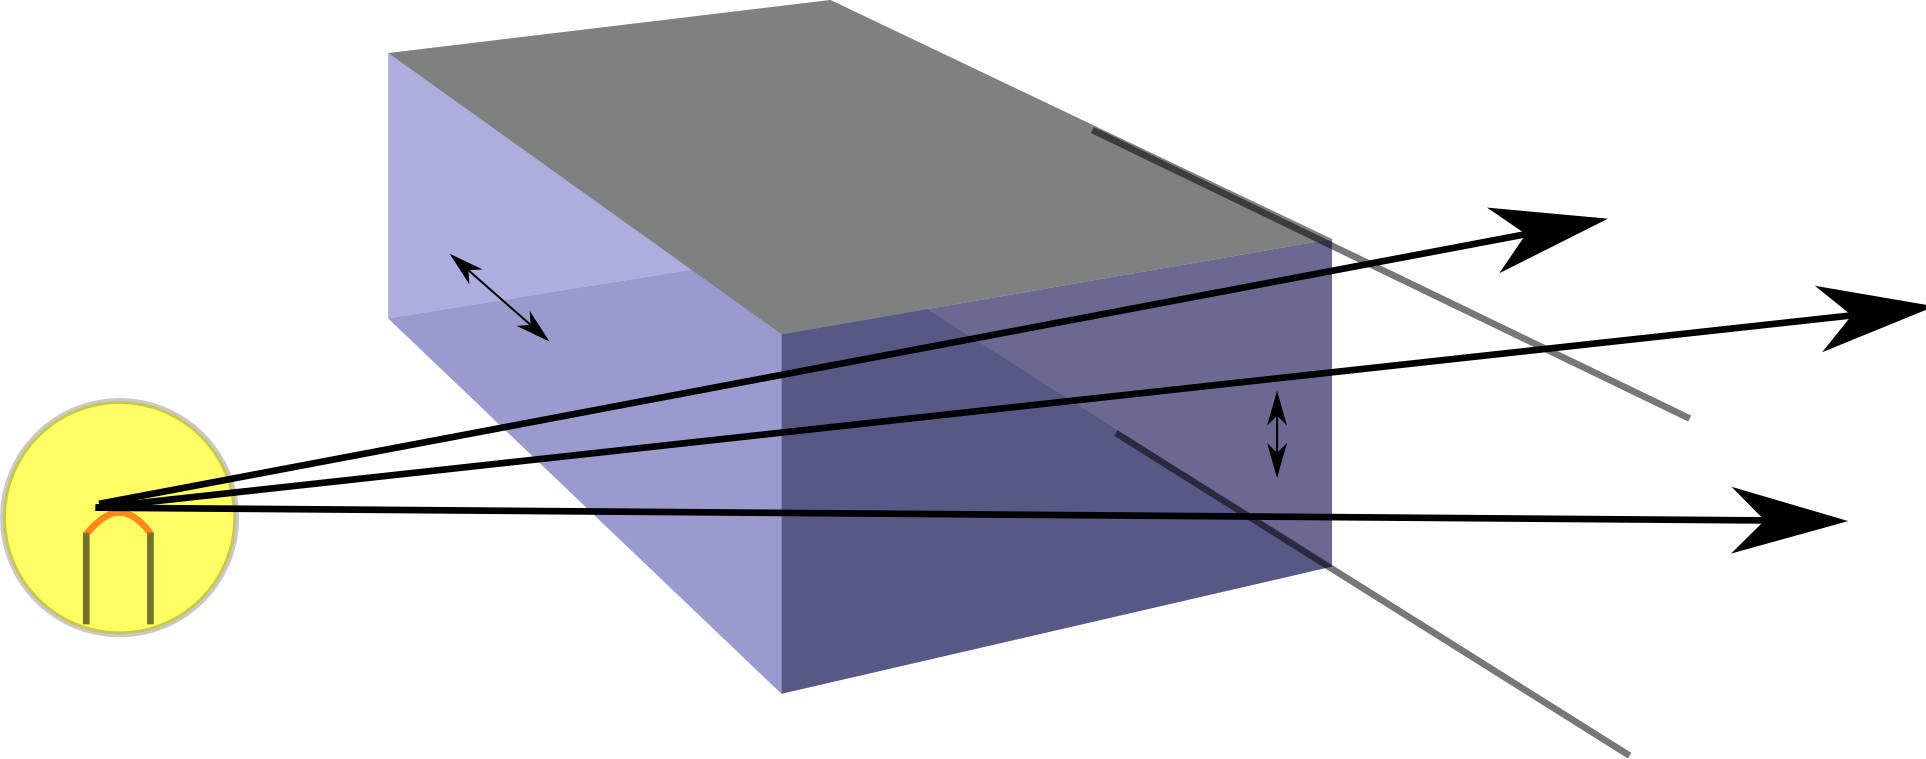
\includegraphics{./kerr}
\end{center}
}
\end{problem}
\begin{problem}
Придумайте способ получения циркулярно поляризованной волны в радиочастотном диапазоне, используя лишь эктронные компоненты.
\end{problem}
\begin{problem}
Известно, что у большинства веществ, например у стекла, магнитная и электрическая проницаемость положительны. Особый интерес в оптике представляет плазма, так как на частотах меньше собственной\footnote{см. умную книжку} электрическая её проницаемость меньше нуля. Однако, уравнения Максвелла и уравнения связи не теряют смысл и при одновременной отрицательности как магнитной, так и электрической проницаемостей вещества. Начертите картину прохождения лучей света через двояковогнутую линзу из вещества с $\varepsilon<0$ и $\mu<0$ одновременно. Попытайтесь найти другие интересные свойства таких веществ.
\end{problem}
\clearpage
%chapter three
\chapter{Механика}
\thispagestyle{empty}
\clearpage
\begin{problem}
C наклонной плоскости с высоты $h$ соскальзывает брусок. В начальной точке он покоится и его энергия равна потенциальной: $\left.E_p\right|_{t=0}=mgh$. В конечной точке брусок приобретает горизонтальную скорость $v$, соответственно его энергия равна кинетической: $\left.E_k\right|_{t}=\frac{mv^2}{2}$, потенциальная энергия равна нулю. Перейдем в систему отсчета, движущуюся относительно первой со скоростью v (скорость бруска в конечной точке пути). Тогда в начальной точке его энергия равна сумме кинетической энергии и потенциальной $\left.E_p\right|_{t=0}=\frac{mv^2}{2}+mgh$. В конечной точке и кинетическая и потенциальная энергии обращаются в ноль. Куда делась энергия?
\end{problem}
\clearpage
\end{document}